% Graphviz writes PDF 1.7; allow it for the included figures
\pdfminorversion=7
% openany: chapters, the contents and the lists start on the next
% page instead of the next odd page, so no blank pages are inserted
\documentclass[openany]{tietreport}

% Import images
\usepackage{graphicx}

% Added for this report: tables and line breaking in long URLs
\usepackage{booktabs}
\usepackage{tabularx}
\usepackage{xurl}

% Bibliography configuration
\usepackage[
  date=year,
  style=alphabetic,
  backend=biber,
  sorting=nty,
  maxnames=5,
  minnames=3,
  maxalphanames=4,
  minalphanames=3,
  backref=true,
  doi=false,
  isbn=false,
  url=true,
  urldate=long,
  eprint=false
]{biblatex}
\addbibresource{references.bib}

% Coloured links instead of boxes, and no headers on blank pages
\usepackage{xcolor}
\definecolor{linkblue}{HTML}{1F4E79}
\hypersetup{colorlinks=true, linkcolor=linkblue, citecolor=linkblue,
  urlcolor=linkblue}
\usepackage{emptypage}

% Ragged-right text in narrow table columns
\newcolumntype{L}{>{\raggedright\arraybackslash}X}
\newcolumntype{P}[1]{>{\raggedright\arraybackslash}p{#1}}

% The class sets 12pt text; fancyhdr needs a slightly taller header
\setlength{\headheight}{15pt}

% Allow larger tables and figures on pages that also have text, so
% that fewer pages are left half empty
\renewcommand{\topfraction}{0.9}
\renewcommand{\bottomfraction}{0.8}
\renewcommand{\textfraction}{0.1}
\renewcommand{\floatpagefraction}{0.8}

% Let long URLs in the bibliography break between characters
\setcounter{biburllcpenalty}{7000}
\setcounter{biburlucpenalty}{8000}

%% ==================================================
%% CUSTOMIZE THESE FIELDS FOR YOUR PROJECT
%% ==================================================

% Course/Lab header
\TitlePageHeader{%
  UCS503 Software Engineering%
}

% Main project title
\ProjectTitle{%
  TripEase%
}

% Subtitle or project description
\ProjectSubTitle{%
  An Integrated Trip Planning and Itinerary Management System%
}

% Student information (up to 4 students)
% (set in a two-column table on the title page below)
\author{%
  \texttt{1024030709} & Nimitt Malhotra \\
  \texttt{1024030712} & Manraj Singh \\
  \texttt{1024030714} & Vatsal Chauhan%
}

% Degree, year, program
\TitlePageSubText{%
  BE Third Year, COE%
}

% Faculty advisor/guide name
\AdvisorName{%
  Ms. Paramveer Sidhu%
}

% Evaluation period and department info
\TitlePageFooterText{{%
    \large Mid-Semester Evaluation \\[0.2cm]
    \bfseries Computer Science and Engineering
    Department%
  } \\[0.15cm]
  Thapar Institute of Engineering and Technology,
  Patiala \\[0.15cm]
  October 2026%
}

%% ==================================================

% Title page with the institute logo. It uses the fields set above;
% only the layout differs from the class: the logo is added at the
% top, the spacing is adjusted so that everything fits on one page,
% and no blank page follows.
\makeatletter
\renewcommand{\maketitle}{%
  \begin{titlepage}
    \centering
    \vspace*{-2.4cm}
    
\includegraphics[width=0.62\textwidth]{figures/tiet-logo.png}\par
    \vspace{1.3cm}
    {\large \textbf{\@tpHeader}\par}
    \vspace{0.1cm}
    {\normalsize Project Report\par}
    \vspace{1.5cm}
    {\LARGE \textbf{\@tpTitle}\par}
    \vspace{0.3cm}
    {\large \@tpSubTitle\par}
    \vspace{1.5cm}
    {\large \textbf{Submitted by:}\par}
    \vspace{0.3cm}
    {\large \begin{tabular}{@{}l@{\hspace{1em}}l@{}}
      \@tpAuthors
    \end{tabular}\par}
    \vspace{0.4cm}
    {\normalsize \@tpSubText\par}
    \vfill
    {\large \textbf{Submitted to:}\par}
    \vspace{0.2cm}
    {\large \@tpAdvisor\par}
    \vspace{1.2cm}
    {\normalsize \@tpFooter\par}
  \end{titlepage}%
}
\makeatother

\begin{document}

% Generate title page
\maketitle

% Table of contents (auto-generated from chapters)
\tableofcontents
\listoffigures
\listoftables

% ===== CHAPTER 1: INTRODUCTION =====

\chapter{Introduction}

\section{Background and Context}

A group of students planning a four-day trip usually ends up
using five tools for it: a search engine and travel blogs to
decide what is worth seeing, a maps app to check whether two
places are near each other, a notes app or shared document for
the day-by-day plan, a spreadsheet for the budget, and a group
chat where all of these are pasted and discussed. None of these
tools share data. When one person changes the plan, the other
copies are out of date, and nobody is sure which version is the
current one.

TripEase is a web application that keeps a trip in one place.
A trip is a single record that holds the cities, the day-by-day
itinerary, the places on a map and the budget. When the
traveller changes one part, the rest is recalculated from the
same record. This report describes the state of the project at
the mid-semester evaluation (October 2026): what we built, how
it is designed, how we tested it and what is still left for the
final submission.

The project is developed by a team of three in a single
repository. The application is in the \texttt{code} folder, the
documentation in \texttt{docs}, and the original proposal in
\texttt{project-proposal}. The detailed documents that this
report summarises (requirements, diagrams, data model and use
cases) are kept in \texttt{docs} and published as a
documentation site.

\subsection{Problem Statement}

The problem is not a lack of tools but the fact that the tools do
not share state. In our proposal we listed the pain points we
had seen in our own group trips:

\begin{itemize}
  \item \textbf{No single source of truth.} The itinerary exists
    in several places at once and the copies disagree.
  \item \textbf{Geography is separate from the plan.} The order of
    the day is decided in a text document, so nothing warns the
    group that two stops are on opposite sides of the city.
  \item \textbf{Manual arithmetic.} The budget is re-totalled by
    hand every time the plan changes.
  \item \textbf{Lossy sharing.} A plan sent as a message goes
    stale as soon as anyone edits the original.
\end{itemize}

\begin{table}[!htbp]
\centering
\small
\caption{Project objectives and their status at the
  mid-semester evaluation.}
\label{tab:objectives}
\begin{tabularx}{\textwidth}{@{}P{0.4cm}LLP{1.5cm}@{}}
\toprule
\textbf{\#} & \textbf{Objective} & \textbf{How it is checked} &
  \textbf{Status} \\
\midrule
1 & A signed-in user can turn a destination, dates, a budget,
    the number of travellers and travel styles into a complete
    multi-day trip with cities, hotels, meals, activities and a
    categorised budget, stored as one record that only this user
    can read. &
    The trip wizard works end to end, also with no external API
    keys (demo providers). Security rules tests in CI. &
    Done \\
2 & Every plan is checked against the clock and the money: each
    day is measured against a 09:00 to 21:00 window, and the
    budget is recalculated after every edit. &
    Feasibility engine and planning tests; manual check in the
    roadmap and budget views. &
    Done \\
3 & A generated trip can be edited in place (activities, hotels
    and cities) without starting again, and every edit is saved
    as soon as it is made. &
    Edit flows in the trip page; city editing tests. &
    Done \\
4 & Every push runs lint, unit tests, the security rules tests
    and a production build, and every merge into \texttt{main}
    is deployed to a staging site. &
    GitHub Actions workflow and Vercel deployment. &
    Done \\
5 & Median time to complete an itinerary (TTCI) of 15 minutes
    or less for first-time users on a 3-day trip with at least 5
    stops. &
    Pilot study with 12 to 20 classmates, against their usual
    tools. &
    Planned \\
6 & Expense logging with a planned-versus-actual view, and a
    read-only link for sharing a trip. &
    Functional requirements FR-25 and FR-26. &
    Planned \\
\bottomrule
\end{tabularx}
\end{table}

Stated formally, the aim is to design and build a web-based
system in which a user assembles a multi-day trip (destinations,
an ordered day-wise itinerary, the places on a map and a
categorised budget) as a single persistent record, and which
reduces the time and the number of separate tools needed to
reach a complete itinerary.

\section{Project Objectives}

Table~\ref{tab:objectives} lists the objectives we are working
to, how each one is checked and where it stands at the
mid-semester point. Objectives 1 to 4 concern the product and
the engineering process. Objectives 5 and 6 are the remaining
work for the final evaluation.


\section{Changes Since the Proposal}

Some parts of the design changed while we built the prototype.
Table~\ref{tab:changes} lists the changes and the reason for each.
The largest is the use of an AI model. The proposal kept
AI-generated itineraries out of scope. We now use a model for one
narrow decision, how many days to spend in each city, because
the rule-based planner can only split a trip sensibly for
destinations we have prepared data for. For any other destination
it puts the whole trip in a single base city. The model does not
choose places or prices, and its answer is checked by our own
rules before it is used (Section~\ref{sec:planning}).

\begin{table}[!htbp]
\centering
\small
\caption{Differences between the proposal and the current
  prototype.}
\label{tab:changes}
\begin{tabularx}{\textwidth}{@{}LLL@{}}
\toprule
\textbf{Proposal} & \textbf{Current prototype} &
  \textbf{Reason} \\
\midrule
The user searches for places and adds them to the trip one by
one. &
The system generates a full itinerary from a places provider,
and the user edits it. &
We expect a generated draft to be quicker to correct than an
empty plan is to fill. The pilot will test this. \\
AI-generated itineraries out of scope. &
An AI model suggests only the split of days between cities. Our
checks validate it and a rule-based planner replaces it on any
failure. &
The rule-based planner cannot split unknown destinations into
several cities. \\
Google Maps for the map, Directions API for routes. &
Leaflet with OpenStreetMap tiles. Travel times are estimated from
distance. &
The map has to work in demo mode, where there are no API keys. \\
A nearest-neighbour ordering offered as a suggestion. &
Stops are ordered nearest-first from the hotel when the day is
generated. The user can reorder them by drag and drop. &
The ordering is applied once, at generation, and stays
overridable. \\
Itinerary items and expenses as Firestore subcollections. &
The whole trip, including its days and activities, is one
Firestore document. &
A trip is small, so one read loads it and one write saves it
(Section~\ref{sec:datamodel}). \\
TTCI instrumentation in iteration 2. &
Not built yet. &
Moved to the pilot work for the final evaluation. \\
\bottomrule
\end{tabularx}
\end{table}

% ===== CHAPTER 2: METHODOLOGY & DESIGN =====

\chapter{Methodology and Design}

\section{Development Process}

We work in iterations. Each iteration is developed on its own
branch, named after its number and topic (for example
\nolinkurl{iteration4-ai-city-planner}), and merged into
\texttt{main} when it works. Documentation and tests are added
through pull requests. Continuous
integration was set up in the first iteration, before the feature
work grew: every push and pull request runs lint, the unit tests,
the Firestore security rules tests against the emulator and a
production build, and a separate job scans the history for
committed secrets. Every merge into \texttt{main} is deployed
automatically to a staging site on Vercel.

Table~\ref{tab:iterations} shows what each iteration delivered
and when it reached \texttt{main}, taken from the repository
history.

\begin{table}[!htbp]
\centering
\small
\caption{Iterations and the date each one was merged into
  \texttt{main}.}
\label{tab:iterations}
\begin{tabularx}{\textwidth}{@{}P{3.2cm}P{2.1cm}L@{}}
\toprule
\textbf{Iteration} & \textbf{Merged} & \textbf{Delivered} \\
\midrule
1 & 31 Aug 2026 & Sign-up and sign-in, creating, listing,
  renaming and deleting trips, adding named places to a trip,
  Firestore security rules with tests, continuous integration. \\
Planning experience & 5 Sep 2026 & Trip wizard, itinerary
  generation, roadmap with activity and hotel editing, and budget
  breakdown. \\
2: real places & 5 Sep 2026 & Places provider interface with a
  demo provider and a Google Places provider; every place records
  its source. \\
3: Google Places and map & 5 Sep 2026 & Place search in the
  activity editor, the places cache and the interactive Leaflet
  map. \\
4: AI city planner & 6 Sep 2026 & City planning with an AI model,
  validation and fallback, the ``Edit cities'' dialog, and API
  routes protected by Firebase ID tokens. \\
5: feasibility & 6 Sep 2026 & Travel time estimates, day
  feasibility warnings, city transfers and nearest-first
  ordering. \\
Map polish & 6 Sep 2026 & Map and place card improvements, with
  tests. \\
Documentation and tests & 11--12 Oct 2026 & Data flow, architecture,
  ER, use case and activity diagrams, requirements document, updated
  READMEs and additional unit tests. \\
\bottomrule
\end{tabularx}
\end{table}

\section{Requirements}

The requirements are written in the classification used in the
course \cite{sommerville2016}: functional requirements,
non-functional requirements split into product, organisational
and external requirements, and domain requirements. Every
requirement has an identifier so that it can be traced to a use
case and a test. Table~\ref{tab:reqsummary} summarises them. The
full list is in \texttt{docs/requirements.md}.

\begin{table}[!htbp]
\centering
\small
\caption{Summary of the requirements.}
\label{tab:reqsummary}
\begin{tabularx}{\textwidth}{@{}Lrrr@{}}
\toprule
\textbf{Group} & \textbf{Total} & \textbf{Done} &
  \textbf{Planned} \\
\midrule
Functional (FR-1 to FR-27) & 27 & 24 & 3 \\
Non-functional, product (NFR-1 to NFR-11) & 11 & 9 & 2 \\
Non-functional, organisational (NFR-12 to NFR-14) & 3 & 3 & 0 \\
Non-functional, external (NFR-15 to NFR-17) & 3 & 2 & 1 \\
Domain (DR-1 to DR-5) & 5 & 5 & 0 \\
\bottomrule
\end{tabularx}
\end{table}

The three planned functional requirements are expense logging
(FR-25), a read-only share link (FR-26) and recording the time to
complete an itinerary for the pilot (FR-27). The planned
non-functional requirements are the 99\% availability target
during the pilot (NFR-2) and the 15-minute TTCI target (NFR-5).
NFR-17 (privacy) is counted as planned because its pilot part is
not done yet, although the trip part is.

\section{System Architecture}

\subsection{High-Level Design}

Figure~\ref{fig:arch} shows the architecture. TripEase has no
separate backend server. The browser runs the Next.js client,
which signs the user in with Firebase Authentication and reads
and writes the user's own trips in Cloud Firestore directly.
Firestore security rules are the authorisation layer: a trip can
be read or changed only by its owner.

Work that needs a secret key runs in Next.js API routes on the
server: planning the cities, generating and rebuilding an
itinerary, searching for places and serving place photos. These
routes call a shared service layer that holds the planning
pipeline, the itinerary generator, the budget engine, the
feasibility engine and the places providers. The browser uses the
same service layer to recalculate the budget and the feasibility
warnings after an edit, so these are never out of date with the
saved trip. The Google Places and Groq keys are read only on the
server and are never sent to the browser.

\begin{figure}[!htbp]
\centering
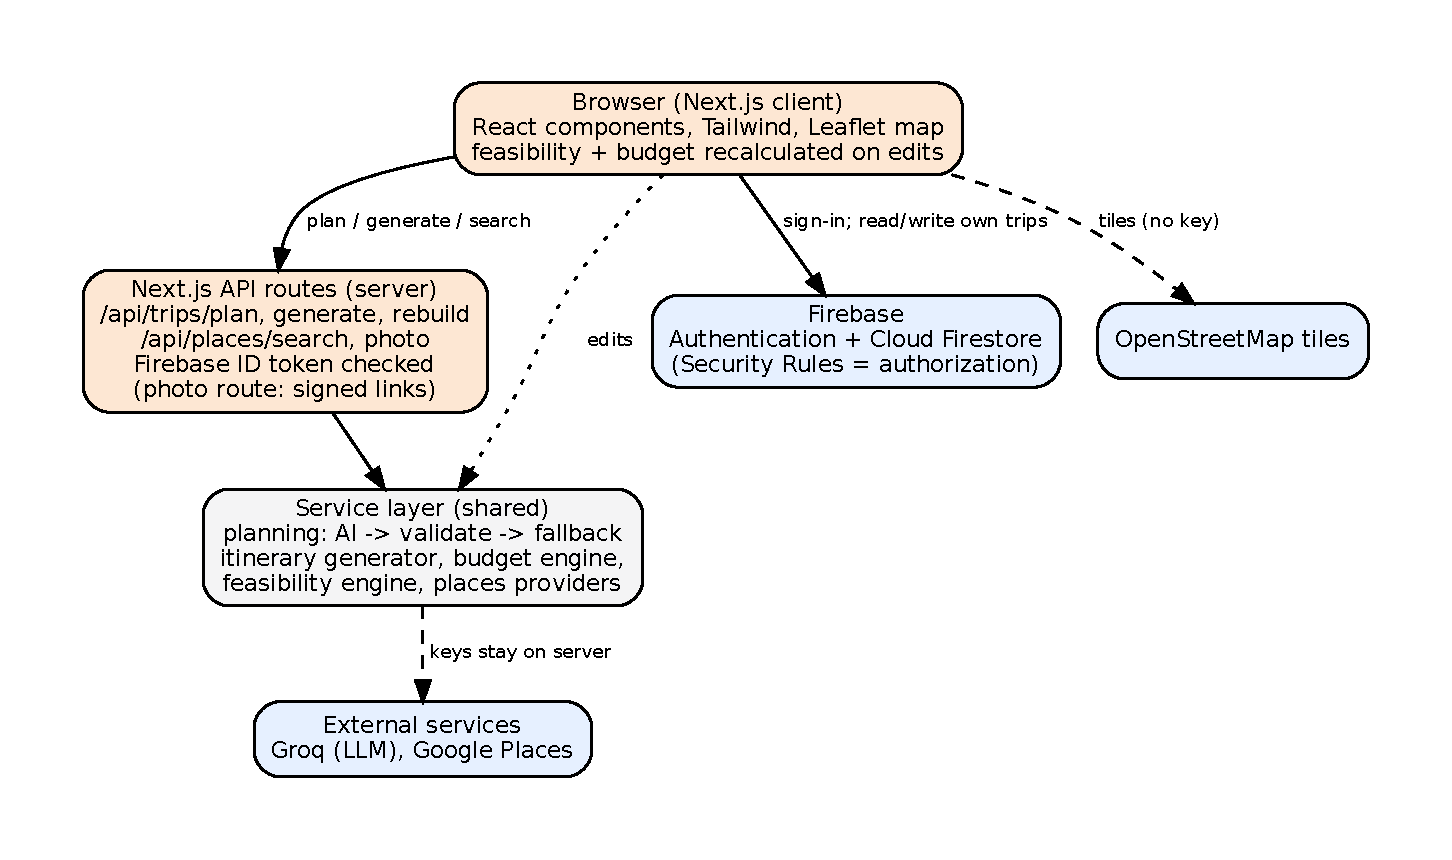
\includegraphics[width=\textwidth]{figures/arch.pdf}
\caption{System architecture.}
\label{fig:arch}
\end{figure}

We chose this design because a separate API server would only
forward requests to the database, and for a three-person team it
would add hosting and security work without a matching benefit.
The cost is dependence on Firebase. To keep that contained, all
database access goes through service files, and the places and AI
providers sit behind interfaces (NFR-10).

\subsection{Data Flow}

Figure~\ref{fig:dfd0} is the context diagram (DFD level 0). It
shows TripEase as one process with five external entities: the
traveller, Firebase Authentication, the places provider (Google
Places), the AI provider (Groq) and the OpenStreetMap tile server.

\begin{figure}[!htbp]
\centering
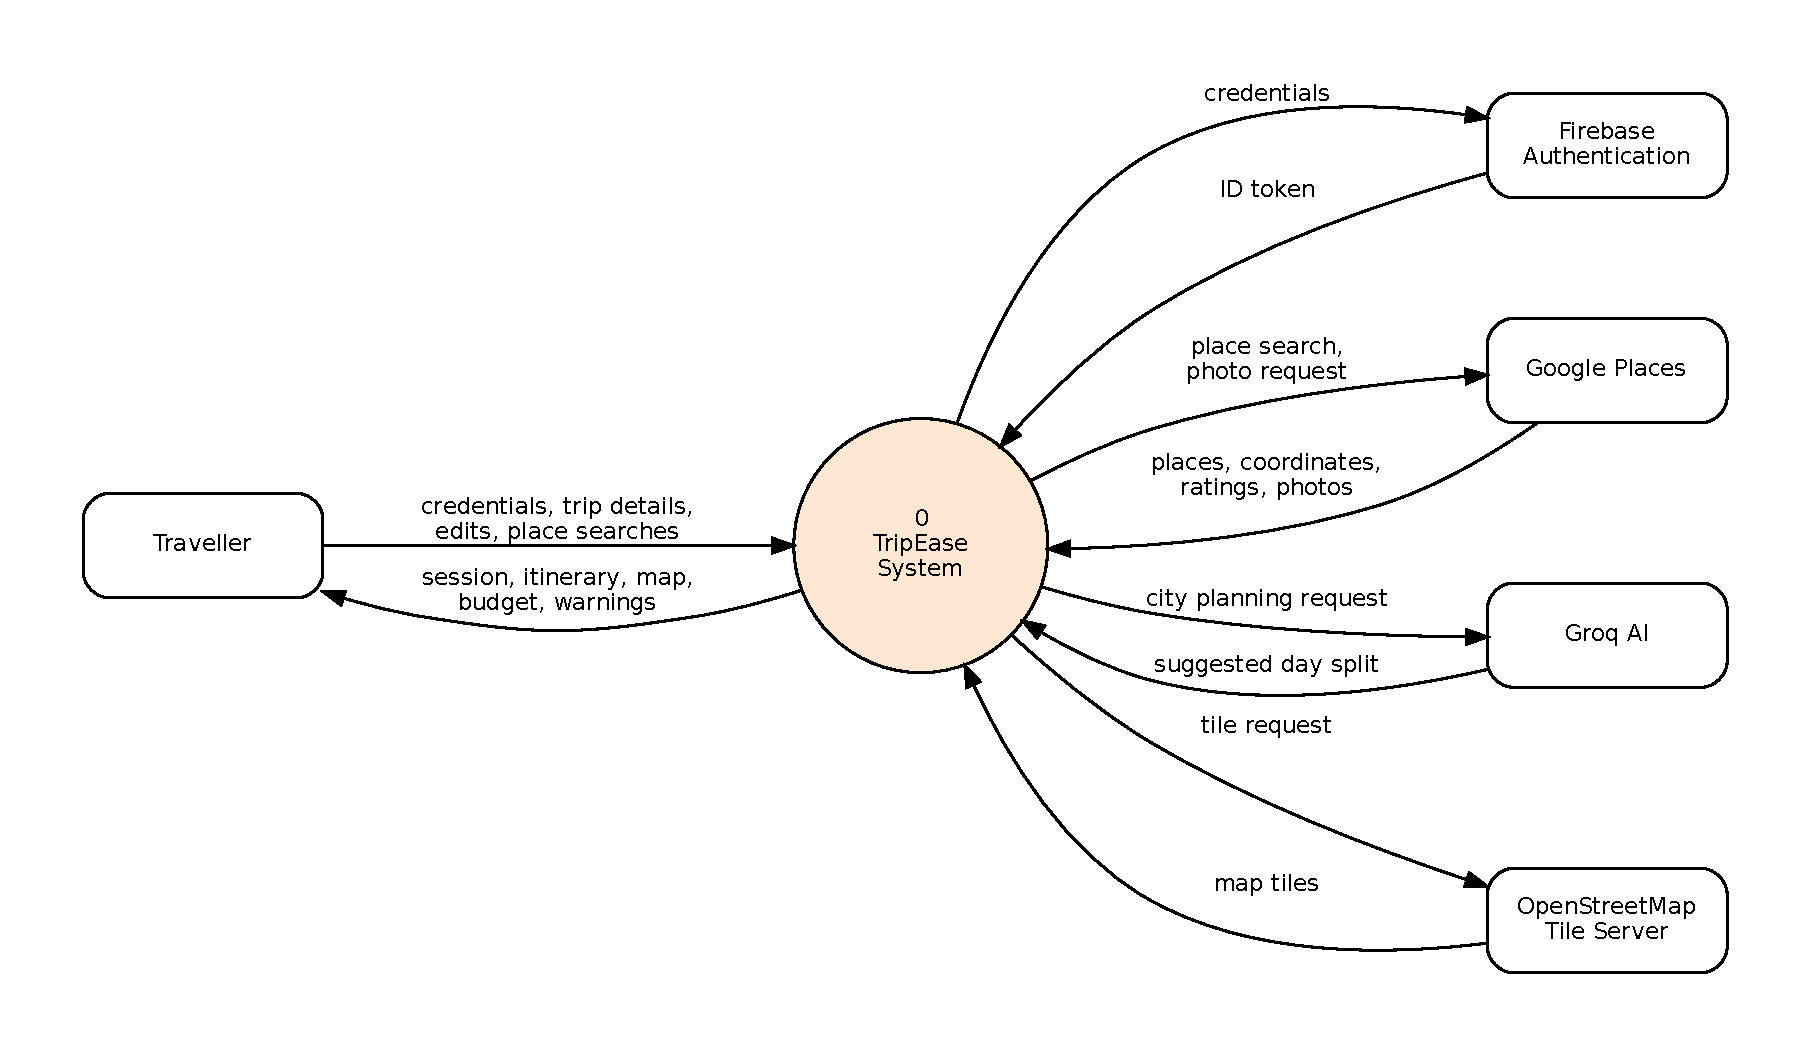
\includegraphics[width=\textwidth]{figures/dfd0.pdf}
\caption{Data flow diagram, level 0 (context diagram).}
\label{fig:dfd0}
\end{figure}

Figure~\ref{fig:dfd1} breaks the system into six processes:
authenticate the user, plan the cities, generate the itinerary,
manage the trip, analyse feasibility, and show the roadmap, map
and budget. There is one data store, D1 Trips. Feasibility is
read from the stored trip and is never written back, which is why
process 5.0 only reads from D1.

\begin{figure}[p]
\centering
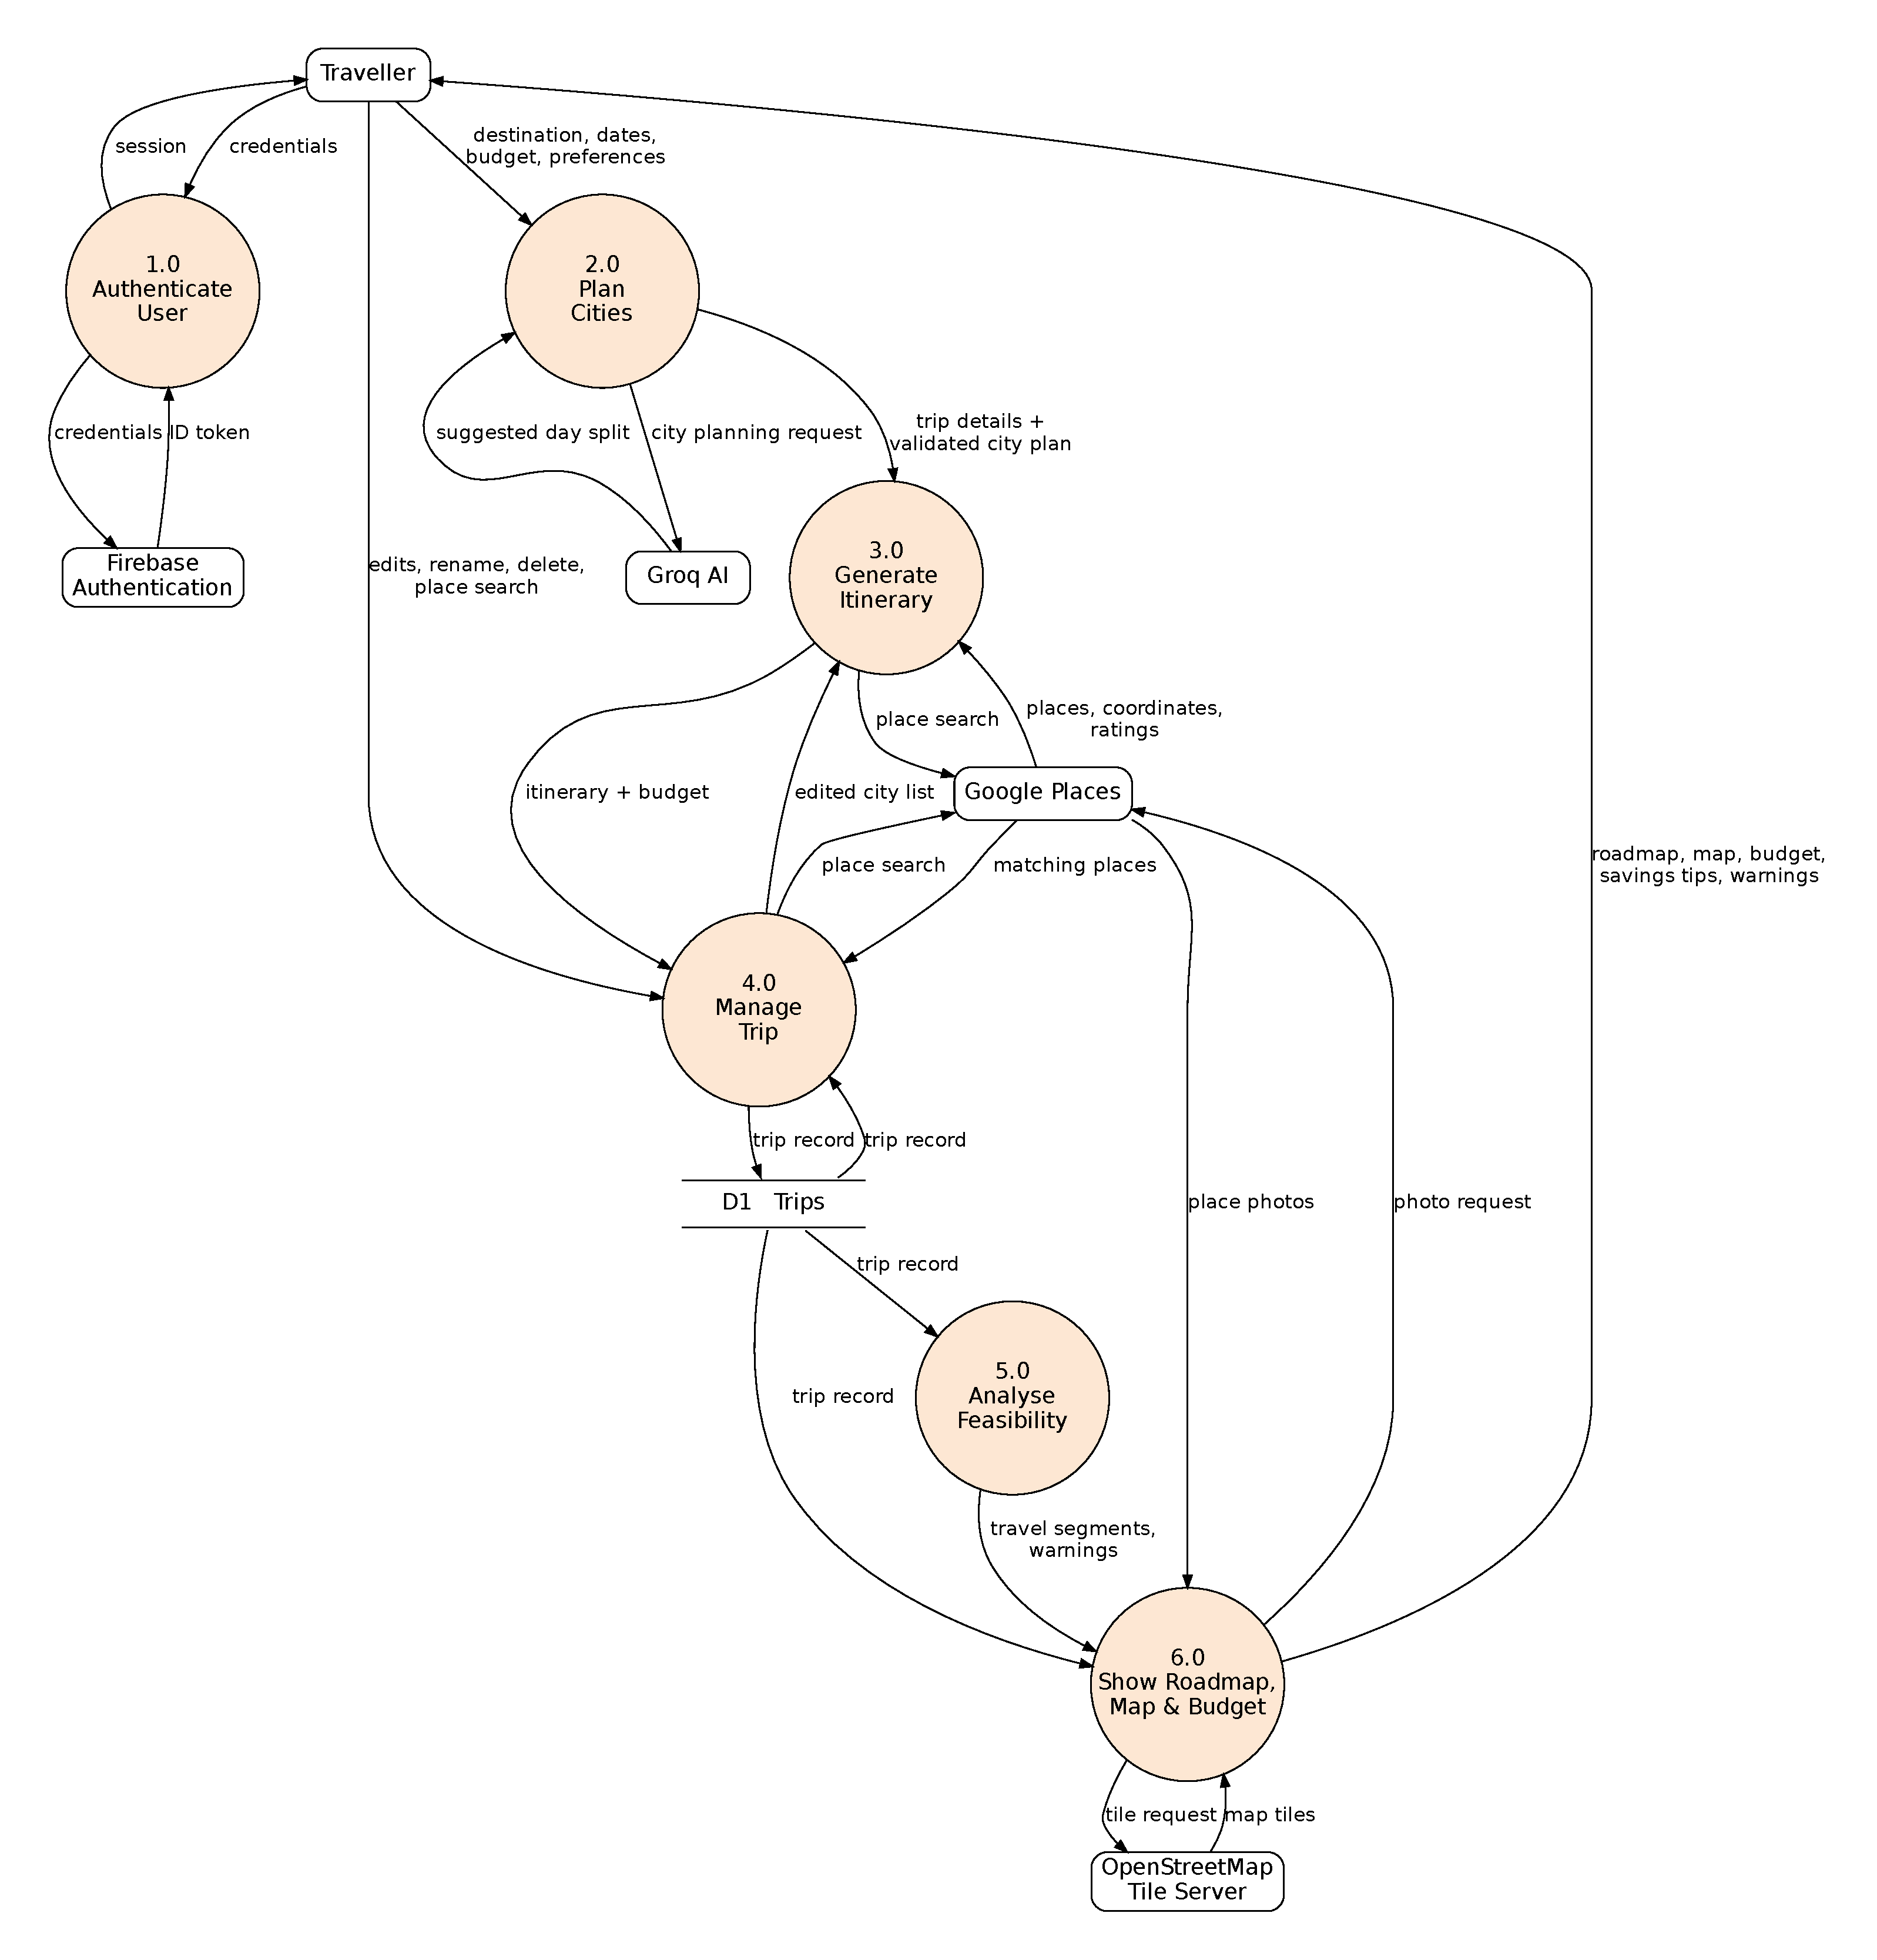
\includegraphics[width=\textwidth]{figures/dfd1.pdf}
\caption[Data flow diagram, level 1.]{Data flow diagram, level 1.
  For the report it is drawn top to bottom; the left-to-right
  version in \texttt{docs/diagrams} has the same processes and
  flows.}
\label{fig:dfd1}
\end{figure}

\subsection{Technical Stack}

\begin{itemize}
  \item \textbf{Framework/Language:} Next.js 16 (App Router) with
    React 19 and TypeScript 5 \cite{nextjs}.
  \item \textbf{Database:} Cloud Firestore for trips, Firebase
    Authentication for accounts (email and password, and Google
    sign-in) \cite{firestorerules}.
  \item \textbf{Tools:} Vitest for unit tests \cite{vitest}, the
    Firebase emulator for the security rules tests, ESLint, GitHub
    Actions for continuous integration, Vercel for deployment,
    Graphviz for the diagrams and MkDocs for the documentation
    site.
  \item \textbf{Libraries:} Tailwind CSS 4 and Radix UI for the
    interface, Leaflet with OpenStreetMap tiles for the map
    \cite{leaflet,osmtiles}, dnd-kit for drag and drop, Recharts
    for the budget chart, Zod for validating input and generated
    data \cite{zod}, and jose for verifying Firebase ID tokens.
  \item \textbf{External services:} Google Places API (New) for
    place data \cite{placestextsearch} and Groq for the city
    planning model \cite{groqstructured}. Both are optional: with
    no keys the app uses built-in demo providers.
\end{itemize}

\section{Data Model}
\label{sec:datamodel}

Figure~\ref{fig:er} shows the logical data model as an ER diagram
in Chen notation \cite{chen1976}. There are eight entities. A
User owns Trips. A Trip contains Cities and has Trip Days, and
each Trip Day is hosted by one City and includes Activities. A
City stays at one Hotel. A Trip has exactly one Budget and may
have one City Plan, which records whether the cities were chosen
by the AI or by the rule-based planner. Hotel, Budget and City
Plan are weak entities, because none of them has an identifier of
its own.

\begin{figure}[!htbp]
\centering
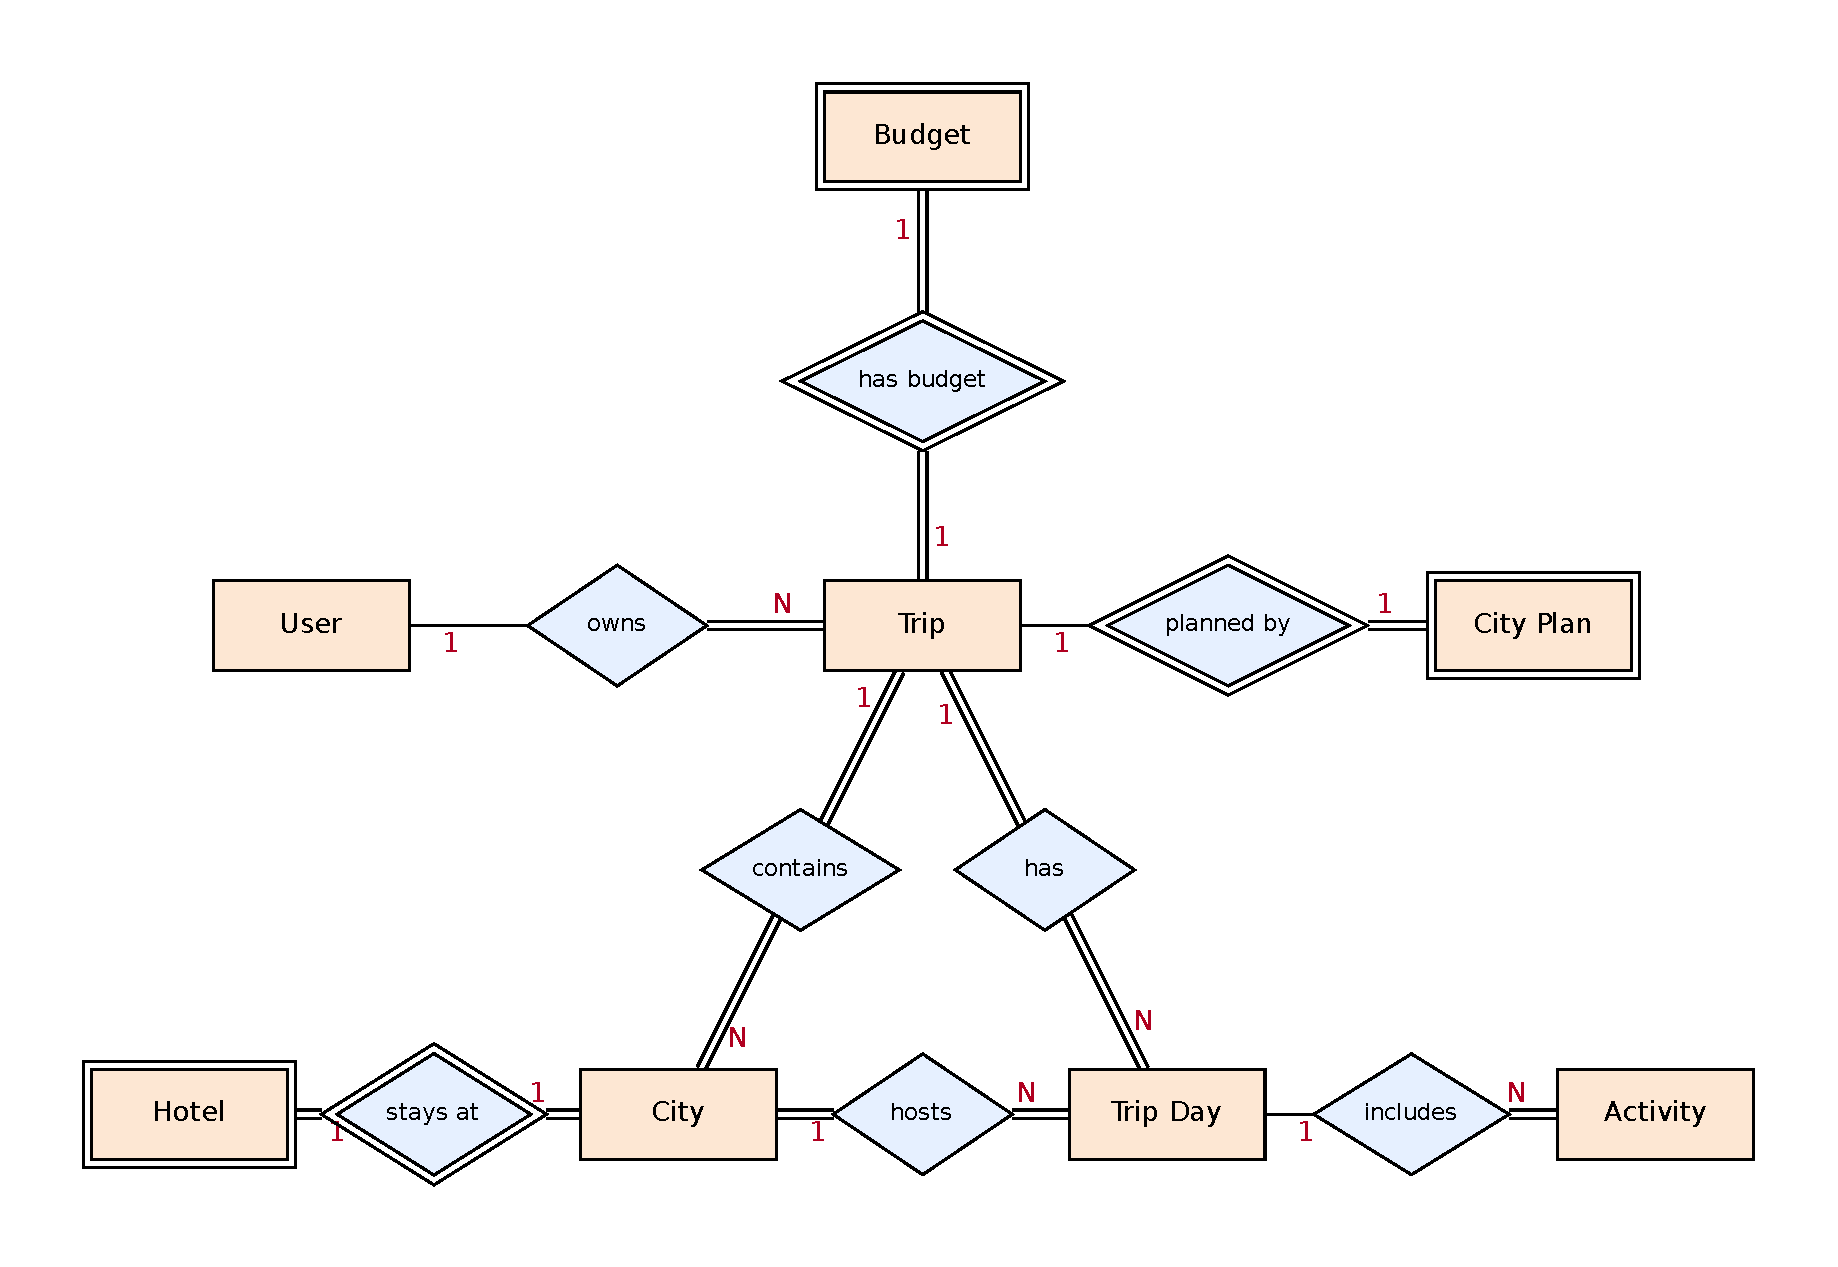
\includegraphics[width=0.92\textwidth]{figures/er-overview.pdf}
\caption[ER diagram (Chen notation).]{ER diagram (Chen notation),
  entities and relationships only. The version with all attributes
  is in \texttt{docs/data-model.md}.}
\label{fig:er}
\end{figure}

In Firestore a whole trip is stored as one document,
\verb|trips/{tripId}|, with the cities, days, activities,
budget and city plan nested inside it. A trip has a handful of
cities and a few dozen activities, so it stays far below the
1~MiB document limit, and the trip page loads it with one read.
The cost is that editing one activity writes back the whole list
of days and the budget, which is acceptable at this size. The
user account is not stored in Firestore at all: it lives in
Firebase Authentication, and a trip refers to it through
\texttt{ownerId}. Values that can be worked out at any time, such
as travel segments, feasibility warnings and savings suggestions,
are computed when the page is drawn and are never saved.

\section{Use Cases}

Figure~\ref{fig:usecase} is the use case diagram, drawn in the
notation from the course \cite{booch2005}. The traveller is the
only human actor. Firebase Authentication, Cloud Firestore, the AI
provider, the places provider and OpenStreetMap take part as
other systems. UC-1 to UC-7 are the main use cases from the
requirements. UC-8 to UC-12 are supporting use cases that the
main ones include or extend: for example, creating a trip always
includes planning the city split (UC-8), fetching places (UC-10)
and working out the budget and saving the trip (UC-11), while the
fallback planner (UC-9) extends UC-8 only when the AI cannot be
used. Each use case is written out in the course template, with
typical, alternate and exceptional flows, in
\texttt{docs/use-cases.md}.

\begin{figure}[p]
\centering
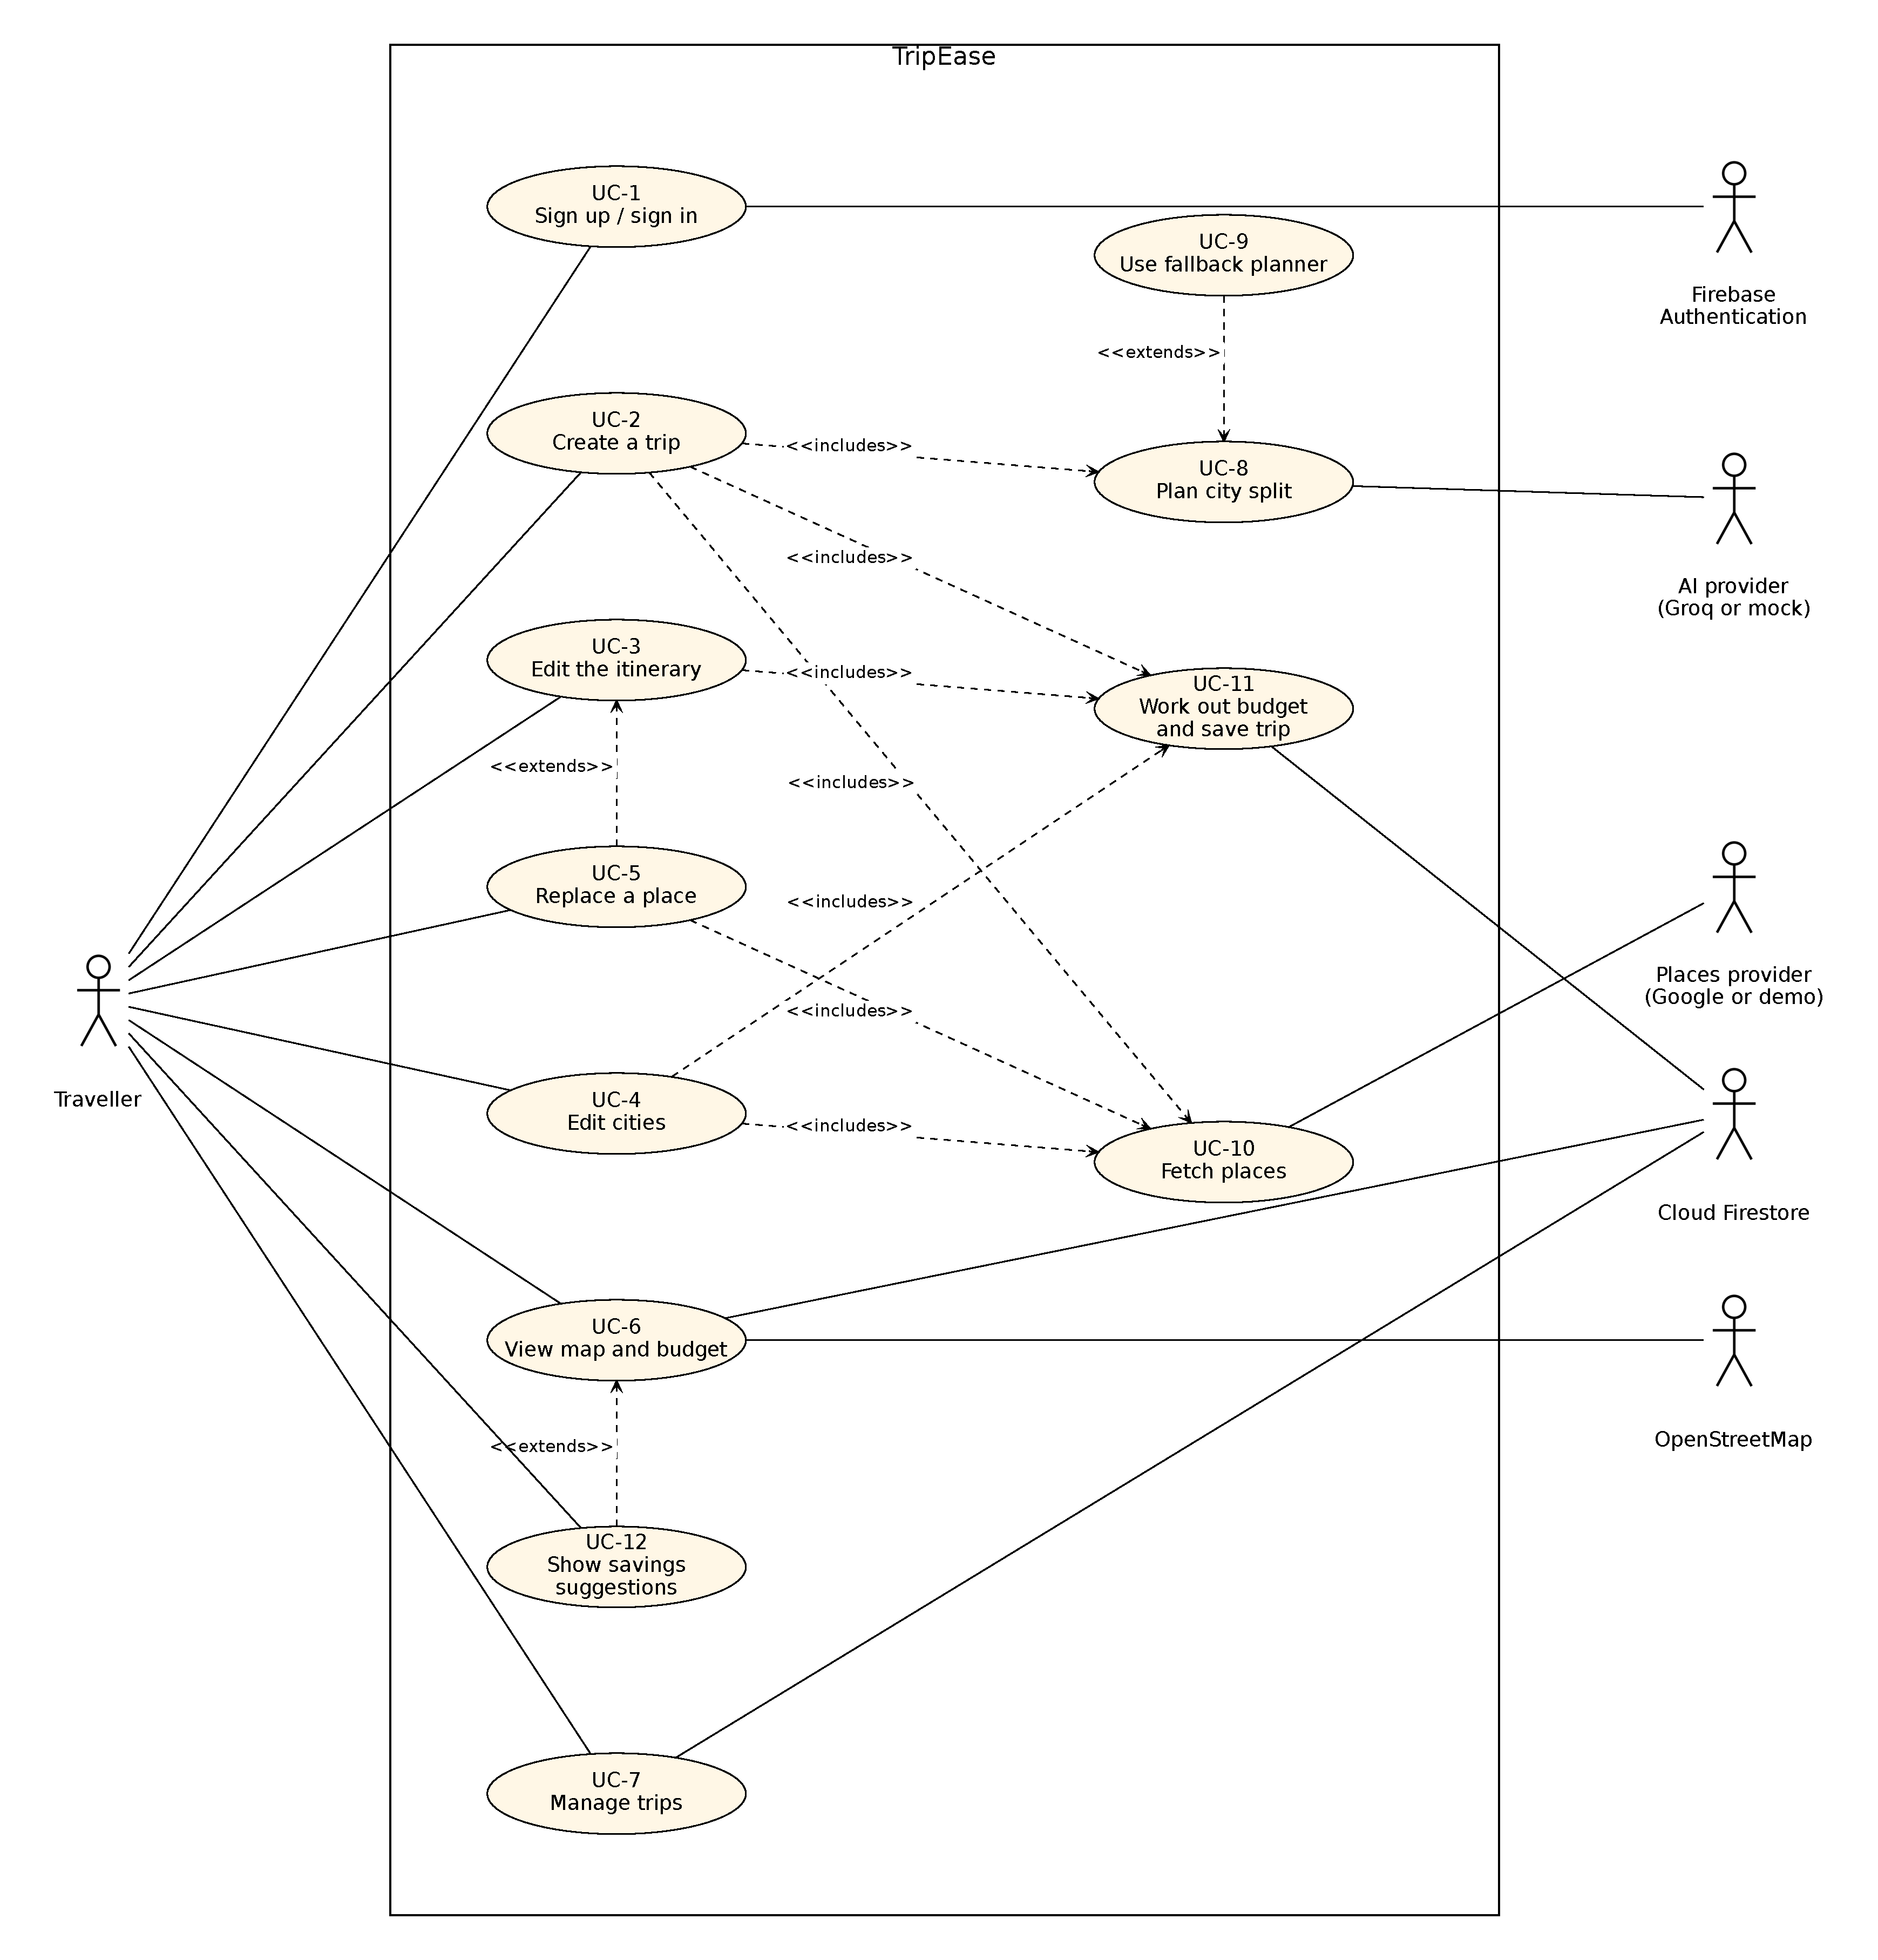
\includegraphics[width=\textwidth]{figures/usecase.pdf}
\caption{Use case diagram.}
\label{fig:usecase}
\vspace{0.1\textheight}% counts towards the float page, so it gets its own page
\end{figure}

\section{Implementation Details}

\subsection{Module 1: Trip Planning Pipeline}
\label{sec:planning}

A trip is created in two steps. First the cities are planned,
then the itinerary is generated for those cities.
Figure~\ref{fig:activity} shows the whole flow, from the traveller
pressing the button to the saved trip, including the retry and the
fallback described below. Its five swimlanes show who performs each
action: the traveller, TripEase, the AI provider, the places provider
and Cloud Firestore. The steps are also described one by one in
\texttt{docs/activity-diagram.md}.

\begin{figure}[p]
\centering
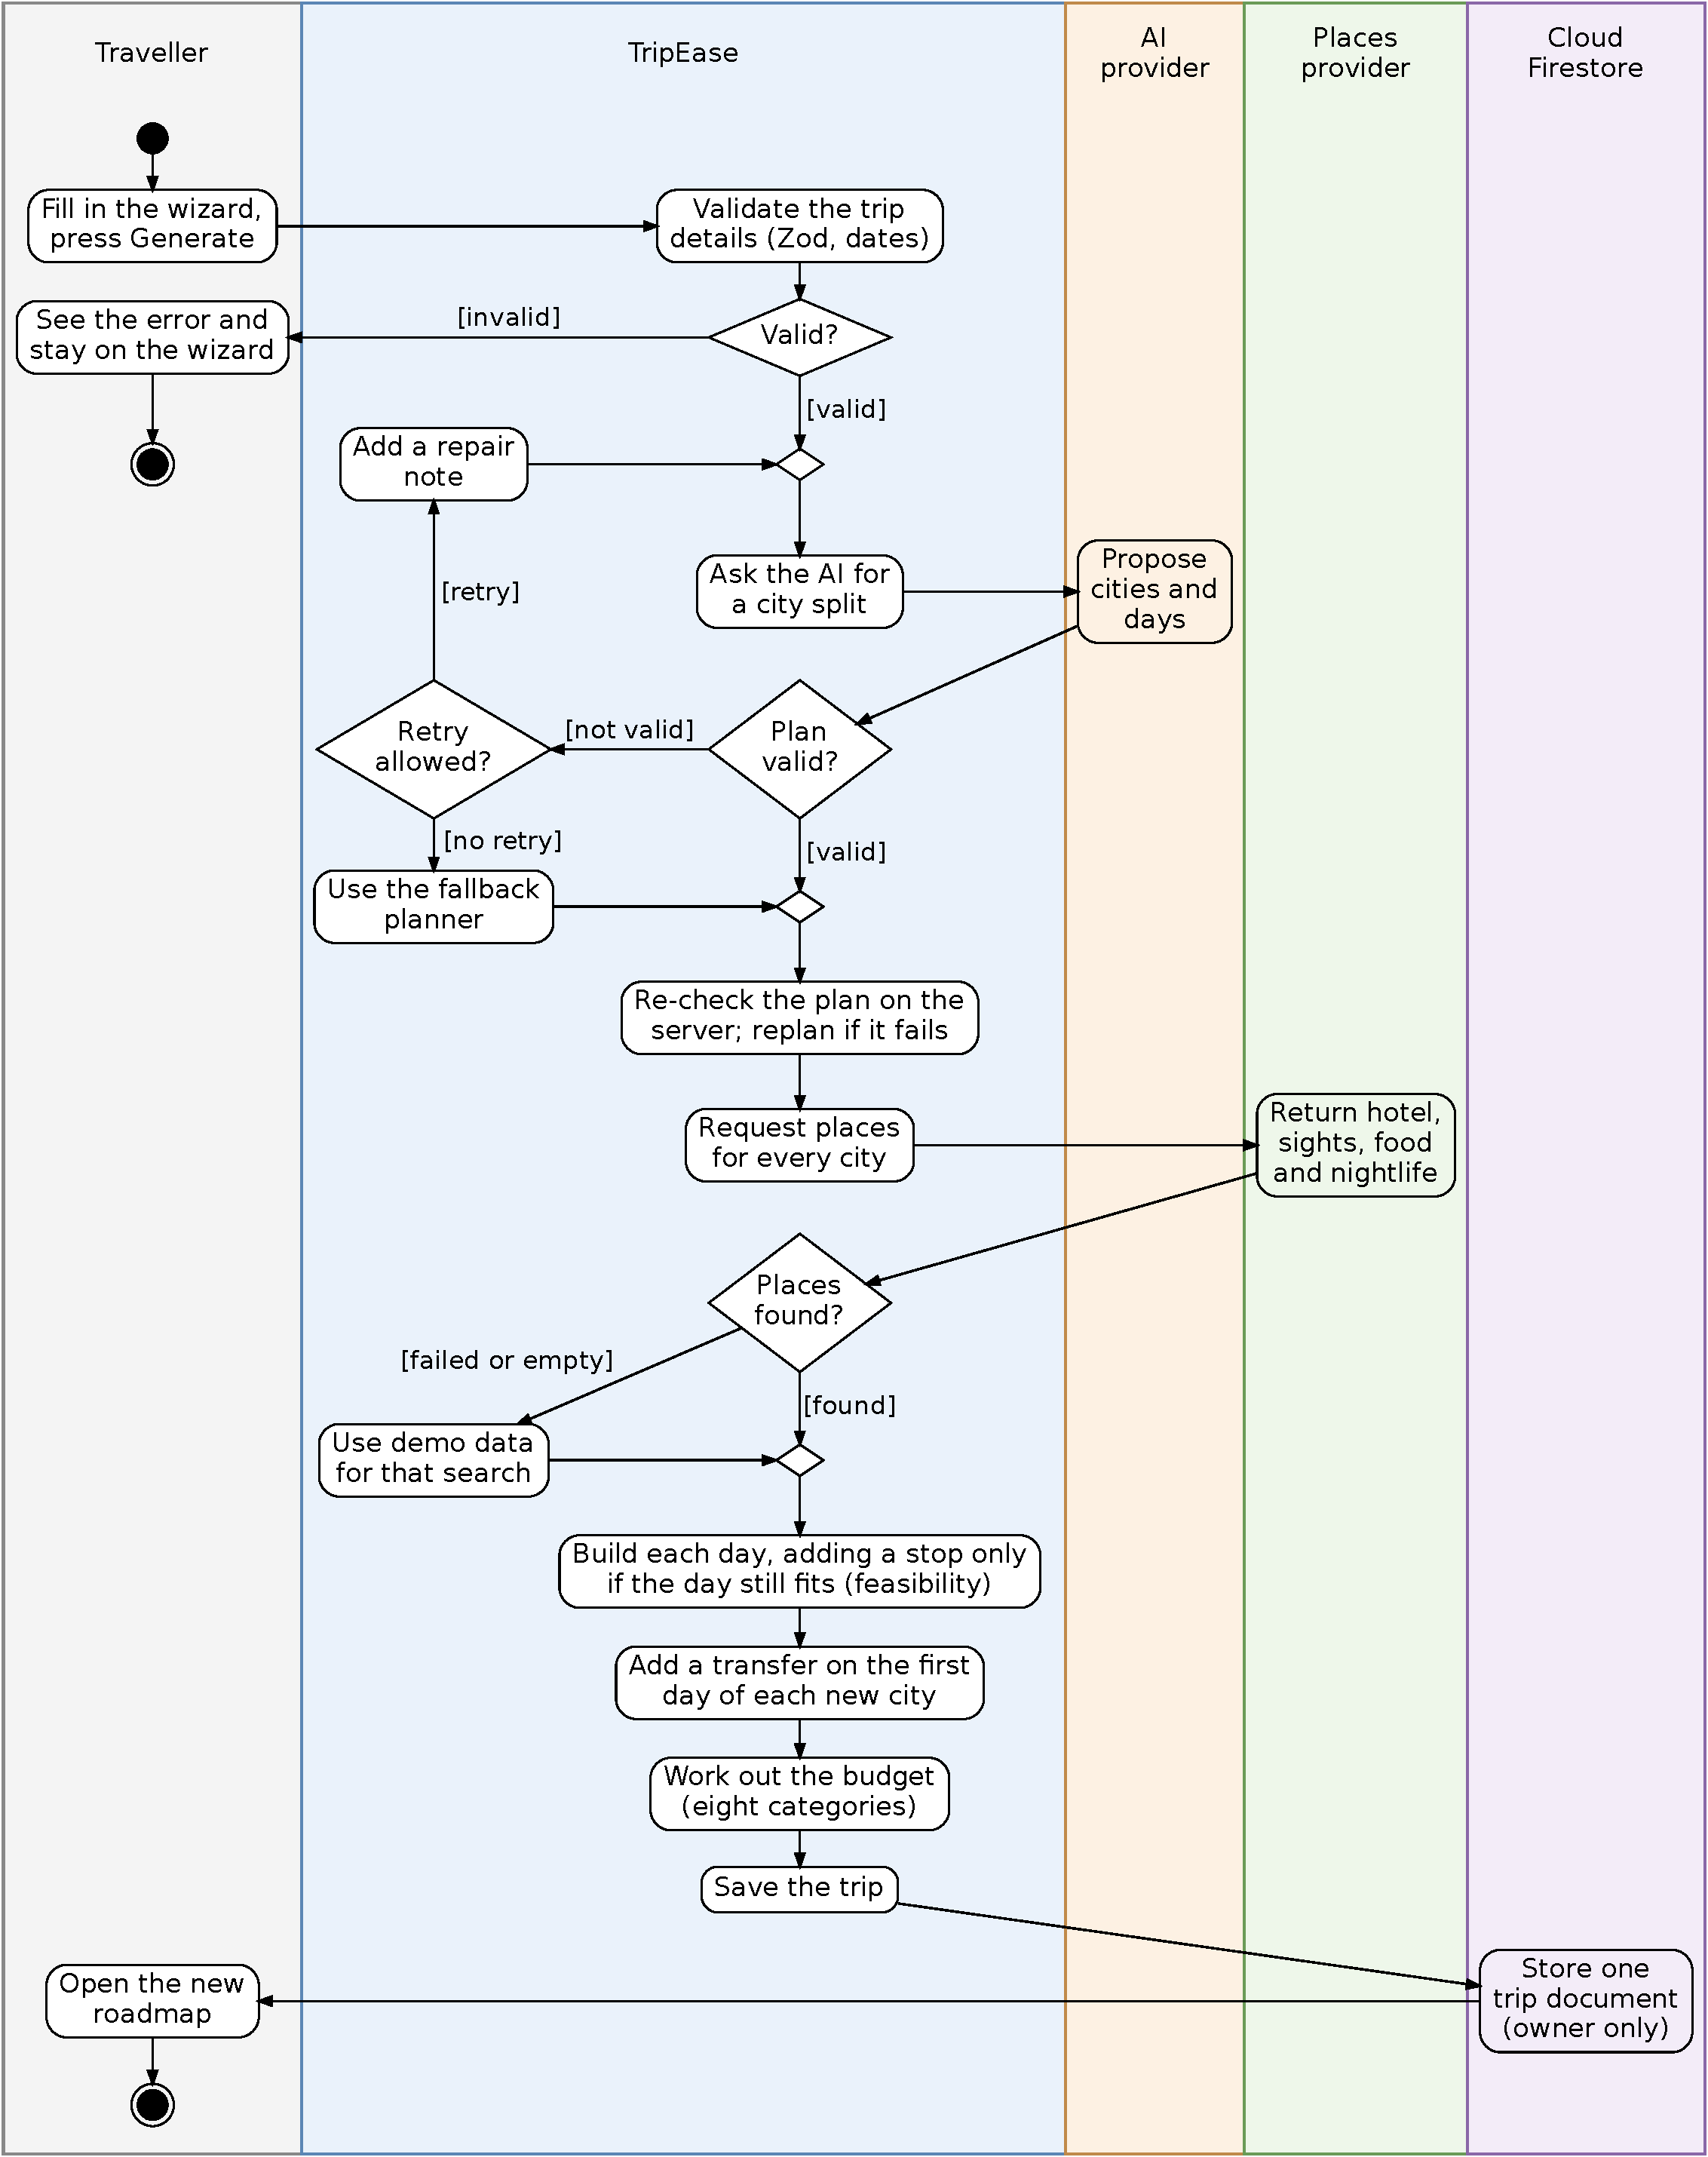
\includegraphics[width=\textwidth,height=0.94\textheight,keepaspectratio]{figures/activity.pdf}
\caption{Activity diagram of creating a trip (UC-2).}
\label{fig:activity}
\end{figure}

\paragraph{City planning.} The server sends the trip details to
the AI provider and asks only for a list of cities, the number of
days in each and a short reason. Where the model supports it, the
answer is constrained to a JSON schema \cite{groqstructured}. The
answer is then checked in two layers. Zod checks its shape, and
our own rules check that it is possible: the plan must be for the
requested destination, the days must add up to the length of the
trip, no city may repeat, every city needs at least one day, and
there can be at most eight cities and no more cities than days.
If the answer is malformed or breaks a rule, the model is asked
once more, with a note on what was wrong. A missing AI key, a timeout
(20 seconds), a quota or authentication error, or a second bad
answer sends the request to the rule-based planner, which always returns a valid
plan. The trip records which planner produced its cities, and a
mock provider used for testing is recorded as the rule-based
planner, not as AI. The traveller therefore always gets a trip,
whether or not the model is available.

\paragraph{Itinerary generation.} For each planned city the
generator asks the places provider for hotels, attractions,
restaurants and nightlife: four searches per city, which a test
keeps fixed because each search is billable in Google mode. It
picks a hotel, groups the sights by area so that each day covers
one part of the city, orders the stops nearest-first from the
hotel, and adds meals. A stop is added to a day only if the day
still fits the time window with dinner held in reserve, using the
same arithmetic as the feasibility engine, so the generator does
not produce days that the engine would then mark as impossible.
The result is validated with Zod before it is returned.

\paragraph{Places providers.} Places come from one interface with
two implementations: a demo provider with curated data for
Thailand and a generic template for other destinations, and a
provider for the Google Places API (New) Text Search
\cite{placestextsearch}. If a live search fails or returns
nothing, the gap is filled from the demo provider instead of
failing the whole trip. Every place keeps its source, and a place
without a verifiable source is labelled ``Demo data''. Live
answers are cached on the server for 10 minutes, with at most 500
entries, so that the same search is not paid for twice.

\subsection{Module 2: Feasibility Engine}

The feasibility engine answers whether a day can actually happen.
Distances are great-circle (haversine) distances
\cite{sinnott1984}, multiplied by a detour factor of 1.3 for road
travel. The travel mode and speed are chosen by distance: within a
city, walking up to 1.2~km and then car; between cities, car,
then train up to 400~km, then flight. Car, train and flight times include a fixed
overhead for getting started (three hours for a flight), so a short
flight is not reported as taking only minutes. A day's total is the time at each place, plus the travel
between them, plus a buffer of 30 minutes and 10 more per stop,
measured against the 09:00 to 21:00 window (720 minutes). A day
over the limit is marked red, and a day with 45 minutes or less to
spare is marked amber. A change of city appears as its own travel
step on the arrival day. All of this is arithmetic over the saved
trip, so it costs no API calls and needs no stored state. All
travel times are labelled as estimates, because no routing
service is used (NFR-16).

\subsection{Module 3: Budget Engine and Savings Suggestions}

The budget engine adds up the trip in eight categories: flights,
hotels, food, activities, transport, shopping, miscellaneous and
an emergency buffer. Hotels are the nightly price times the
nights, activities are added to the category that matches them,
and a fixed daily amount is added for local transport.
Miscellaneous is 4\% of the other costs, and the buffer is 5\% of
the user's budget with a minimum of 3,000. The budget is
recalculated after every edit, so it always matches the plan.

When the estimate is above the budget, the budget tab shows up to
three suggestions, each with its saving: a cheaper hotel in the
city with the most expensive one, a shared tour instead of the
most expensive non-food activity, and local restaurants instead
of hotel dining. Applying a suggestion makes exactly the edit it
describes (for example, the hotel price drops to 70\% and the
hotel is marked as demo data), and the budget is worked out again.
The suggestions are not stored with the trip. The trip page works
them out from the current trip whenever it changes, so they never
go out of date. The rules are simple and fixed, so every suggestion
can be explained.

\subsection{Module 4: Editing and Persistence}

On the trip page the traveller can add, edit, remove and drag
activities, change a city's hotel, and replace an activity with a
real place found through search. Each change is applied to the
trip in the browser, the budget is recalculated, and the
itinerary fields of the trip (cities, days, budget and city plan)
are written to Firestore in one update, together with the time of
the change. Because the page listens to
the trip document, the roadmap, map and budget update as soon as
the write is made.

Editing the list of cities is handled by the server. The dialog
runs the same plan checks as the AI's answer while the traveller
types, and the server checks the list again before rebuilding. A
city that is kept keeps its hotel and its edited activities; only
new or renamed cities, and extra days added to an existing city,
cost a new places lookup. Editing the cities therefore does not
throw away the rest of the traveller's work.

\subsection{Module 5: Security}

Security rules restrict every trip to its owner, deny everything
that is not explicitly allowed, and do not let the owner of a
trip be changed after it is created (NFR-7). The API routes that
spend external quota (plan, generate, rebuild and place search)
require a Firebase ID token and return 401 without one. The
server verifies the token as a JSON Web Token \cite{rfc7519}
against Google's published public keys, as described in the
Firebase documentation \cite{firebaseverify}. This needs no
service-account secret on the server. The trade-off is that a
revoked token is not detected and stays usable until it expires,
which takes at most one hour. The photo route cannot use a bearer
token, because browsers do not send headers for images, so the
server signs each photo link it issues and rejects any link
without a valid signature.

% ===== CHAPTER 3: RESULTS & EVALUATION =====

\chapter{Results and Evaluation}

\section{Testing Methodology}

\begin{itemize}
  \item \textbf{Unit Testing:} The services and the main map
    components have unit tests written with Vitest. There are
    256 tests in 20 files, and all of them pass.
    Table~\ref{tab:tests} groups them by area.
  \item \textbf{Integration Testing:} Some tests run several
    parts together. The planning pipeline is tested end to end
    with an injected mock AI provider that can return a valid
    plan, a plan that breaks the rules, malformed JSON or an
    error. The itinerary generator is run with the demo places
    provider and its output is passed through the feasibility
    engine. The 11 Firestore security rules tests run against the
    Firestore emulator and check that owners can read and change
    their trips while other users and signed-out requests are
    refused. We do not yet have end-to-end tests that drive the
    application in a browser.
  \item \textbf{Performance Testing:} We measured the time taken
    by the parts of trip creation that run on our own code, with
    the demo providers, so that network time is excluded
    (Section~\ref{sec:perf}).
  \item \textbf{User Testing:} Not done yet. The pilot study with
    12 to 20 classmates is planned for the final evaluation.
\end{itemize}

All of these tests except the rules tests run with
\texttt{npm test}. The rules tests run with
\texttt{npm run test:rules}, which needs Java for the emulator.
Both run in continuous integration on every push.

\begin{table}[!htbp]
\centering
\small
\caption{Unit tests by area.}
\label{tab:tests}
\begin{tabularx}{\textwidth}{@{}P{3.6cm}Lrr@{}}
\toprule
\textbf{Area} & \textbf{What is tested} & \textbf{Files} &
  \textbf{Tests} \\
\midrule
City planning & Plan checks, rule-based planner, pipeline with
  retry and fallback, city editing, Groq provider (including
  timeout) & 5 & 46 \\
Itinerary generation and places & Places requests per trip,
  restaurant handling, generated itineraries checked for
  feasibility, places cache & 4 & 36 \\
Feasibility & Distances, travel times, durations, ordering and
  day evaluation & 5 & 84 \\
Map and place display & Map points, map component, place card
  & 3 & 51 \\
Authentication & Firebase ID token verification & 1 & 6 \\
Utilities & Money, duration and date formatting, date arithmetic
  & 2 & 33 \\
\midrule
\textbf{Total} & & \textbf{20} & \textbf{256} \\
\bottomrule
\end{tabularx}
\end{table}

\section{Performance Metrics}
\label{sec:perf}

Table~\ref{tab:perf} shows the measured times. We ran the city
planner, the itinerary generator and the feasibility analysis 50
times each, with the demo providers, on Node.js 22 in a Linux
development environment. We repeated the whole measurement three
times and report the middle of the three medians. Two sample trips
were used: a 9-day trip to Thailand for two travellers, which the
planner split into Bangkok (4 days) and Phuket (5 days) with 43
activities in total, and a 3-day trip to Jaipur for four
travellers with 16 activities. The first run of each step is
slower, because the JavaScript engine has not yet compiled the
code, which is why we report the median and not the mean.

\begin{table}[!htbp]
\centering
\small
\caption[Measured time of the steps that run on our own code.]{Median
  time of the steps that run on our own code (demo providers, 50
  runs).}
\label{tab:perf}
\begin{tabular}{@{}lrr@{}}
\toprule
\textbf{Step} & \textbf{Thailand, 9 days} &
  \textbf{Jaipur, 3 days} \\
\midrule
City planning, rule-based planner & 0.010 ms & 0.005 ms \\
City planning, mock AI provider with checks & 0.033 ms & 0.021 ms \\
Itinerary generation & 0.691 ms & 0.207 ms \\
Feasibility analysis of the whole trip & 0.105 ms & 0.025 ms \\
\bottomrule
\end{tabular}
\end{table}

Our own code takes under a millisecond per trip, so the time
a user waits is set by the external services: the AI call, which
is cut off after 20 seconds (NFR-3), and the place searches, of
which there are four per city and which are cached for 10
minutes (NFR-4). We have not yet measured these with live keys.

The proposal defined a primary metric and several secondary
metrics for a pilot study (Table~\ref{tab:metrics}). None of them
can be measured before the pilot, and we have not changed the
targets.

\begin{table}[!htbp]
\centering
\small
\caption{Evaluation metrics from the proposal.}
\label{tab:metrics}
\begin{tabularx}{\textwidth}{@{}P{4.2cm}LP{2.3cm}@{}}
\toprule
\textbf{Metric} & \textbf{Target} & \textbf{Status} \\
\midrule
Time to complete an itinerary (TTCI) & Median of 15 minutes or
  less for a 3-day trip with at least 5 stops & Pilot \\
Tool count & One tool for the planning task & Pilot \\
Task completion rate & At least 80\% complete the task unaided &
  Pilot \\
Re-order rate after viewing the map & Reported, no target &
  Pilot \\
Perceived clarity & Mean of at least 4 on a 1 to 5 scale & Pilot
  \\
Reliability of sign-in and saving & At least 99\% on staging
  during the pilot & Pilot \\
Delivery cadence & Every iteration ends with a green build on
  staging & To be reported \\
\bottomrule
\end{tabularx}
\end{table}

\section{Analysis}

\paragraph{Objectives.} Objectives 1 to 4 are met. A signed-in
user can create a complete trip from the wizard, edit it in
place, and see the map, the feasibility warnings and the budget
update with each change. The app works end to end with no
external keys. Continuous integration and automatic deployment
are in place. Objectives 5 and 6 (the pilot, expenses and
sharing) are still to be done.

\paragraph{Where the prototype goes beyond the proposal.} The
proposal described a tool in which the user adds every place by
hand. The prototype generates a complete first draft, checks
every day against the clock, and keeps the budget in line with
every edit. It also records where each place came from, so that
demo data and estimated prices are never presented as verified
facts.

\paragraph{Challenges and how we handled them.}
\begin{itemize}
  \item \textbf{AI answers cannot be trusted as they are.} A model
    can return a plan that is well-formed but impossible, such as
    city days that add up to 11 for a 9-day trip. We limited the
    model to one decision, checked its answer with our own rules,
    allowed a single correction round and kept a rule-based
    planner as the fallback.
  \item \textbf{Paid place searches.} An earlier version searched
    for restaurants separately for each meal. We reduced this to
    four searches per city, fixed by a test, and cached the
    results.
  \item \textbf{Plans that cannot happen.} A generated day can
    look fine and still be impossible. The feasibility engine is
    used while a day is being generated as well as when it is
    displayed.
  \item \textbf{Keeping keys secret.} All calls that need a key
    run in server routes that require a signed-in user, and the
    photo route only accepts links that the server has signed.
\end{itemize}

\paragraph{Problems found during this evaluation.} While
preparing this report we checked the prototype against its own
requirements and found three defects, which we are fixing before
the final submission:
\begin{itemize}
  \item The wizard lets the user continue without choosing a
    travel style, but the server requires at least one. The user
    reaches the last step and then sees the error ``Invalid trip
    details.''
  \item Some fixed amounts in the budget are not converted between
    currencies: the daily allowance of 500 for local transport,
    the minimum buffer of 3,000 and the 1,500 threshold for the
    activity savings suggestion. For a trip in US dollars, the
    budget therefore adds 500 dollars a day for local transport. The
    9-day Thailand trip from Table~\ref{tab:perf}, planned in US
    dollars with a budget of USD 1,800, gets an estimate of USD
    9,295, of which USD 4,752 is local transport and USD 3,000 is the
    buffer. The same trip in rupees stays within its
    budget (INR 1,45,965 against INR 1,50,000).
  \item For destinations without prepared data, flights are
    estimated at a default of INR 25,000 per traveller, which is
    far too high for most domestic trips. In the Jaipur example
    from Table~\ref{tab:perf}, four travellers with a budget of
    INR 30,000 get an estimate of INR 1,27,384, of which INR
    1,00,000 is flights.
\end{itemize}
We also found that the budget engine and the code that applies
edits to a trip have no unit tests of their own. Our tests and
demo data are built mainly around Thailand, where the budget
defects above do not show.

% ===== CHAPTER 4: CONCLUSION =====

\chapter{Conclusion}

\section{Summary of Work}

At the mid-semester point, TripEase is a working prototype that
covers the planning part of the problem. A traveller signs in,
answers a short wizard and gets a complete multi-day trip with
cities, hotels, meals, activities, a map and a budget, all kept
in one record that only they can see. They can then change any
part of it, and the map, the feasibility warnings and the budget
follow. The design is documented with data flow, architecture, ER,
use case and activity diagrams and a requirements document. There are 256
unit tests and 11 security rules tests, and they run in continuous
integration on every push. Of the 27 functional requirements, 24
are done. The remaining three (expenses, sharing and recording
the time to complete an itinerary) and the pilot study are the
work for the final evaluation.

\section{Key Findings}

\begin{itemize}
  \item \textbf{Finding 1:} Keeping the AI model to a single,
    checked decision made it optional. Because every answer is
    validated and a rule-based planner is always available, the
    app produces a valid trip with or without the model, and
    with no API keys at all.
  \item \textbf{Finding 2:} The planning, generation and
    feasibility code takes under a millisecond per trip, so the
    waiting time for the user comes almost entirely from the
    external services. Reducing and caching the place searches
    matters more than optimising our own code.
  \item \textbf{Finding 3:} The budget estimates are only as good
    as the fixed amounts and default prices behind them. The
    currency and flight-price defects do not show for Thailand,
    the destination our tests and demo data are built around.
    They became visible only when we looked at a domestic
    destination and at trips in other currencies.
\end{itemize}

\section{Future Work and Recommendations}

\begin{enumerate}
  \item Build expense logging with a planned-versus-actual view
    (FR-25) and a read-only share link (FR-26).
  \item Record the time from creating a trip to completing it
    (FR-27) and run the pilot study to measure TTCI and the
    secondary metrics against the targets fixed in the proposal.
  \item Fix the three defects found in this evaluation: require a
    travel style in the wizard, convert the fixed budget amounts
    into the trip currency, and use realistic flight estimates
    for destinations without prepared data.
  \item Add unit tests for the budget engine and the edit
    functions, and browser-based end-to-end tests for creating
    and editing a trip.
  \item For a real deployment: use a routing service and opening
    hours instead of estimated travel times, move token
    verification to the Firebase Admin SDK if revoked sessions
    must be cut off at once, and move to a paid map tile host,
    since the OpenStreetMap tile service is meant for light use
    \cite{osmtiles}.
\end{enumerate}

\section{Final Remarks}

The main thing we have learned so far is that much of the design
work in this project is about making external services safe to
depend on: checking what they return, deciding what happens when they
fail, and labelling estimates as estimates. The features are only
useful because the app still behaves sensibly when a model, a
key or a search is missing. The second half of the semester is
about measuring whether TripEase actually saves a group time,
which the prototype cannot tell us on its own.

% ===== BIBLIOGRAPHY =====

% Print bibliography with heading in TOC
\printbibliography[heading=bibintoc]

\end{document}
